\chapter{實驗結果與分析}
\label{cha:Evaluation}

此章節中,我們將針對前述第~\ref{cha:Method}~章之研究方法進行實驗結果評估與分析,將說明第~\ref{sec:SystemStructure}~小節之實驗系統架構、第~\ref{sec:DataPreprocessEvaluation}~小節之資料前處理評估、第~\ref{sec:DataAnalysisEvaluation}~小節之資料分析評估、第~\ref{sec:MachineLearningEvaluation}~小節之機器學習評估、第~\ref{sec:PredictionResultAnalysisEvaluation}~小節之預測結果分析評估,以及第~\ref{sec:ApplicationAnalysisEvaluation}~小節之產業應用分析評估。

\section{實驗系統架構}
\label{sec:SystemStructure}

本論文實驗系統架構將分為資料前處理端、資料分析端與機器學習端,如~\ref{tab:ResearchEnvironment},並均以 Python 做為開發語言。

\begin{itemize}
    \item [■] 資料前處理端:以 Apache Spark~\cite{armbrust2015spark}處理資料之前處理以及分割資料集所使用。
    \item [■] 資料分析端:以 missingno~\cite{Bilogur2018}、Seaborn~\cite{michael_waskom_2020_3767070}協助以圖表方式呈現資料特性。
    \item [■] 機器學習端:以 pandas~\cite{jeff_reback_2020_3715232}~\cite{mckinney-proc-scipy-2010}、scikit-learn~\cite{scikit-learn}~\cite{sklearn_api}、XGBoost~\cite{chen2016xgboost}處理機器學習訓練與評估。
\end{itemize}

\begin{table}[!htb]
	\centering
	\begin{tabular}{cclclcl}
	\hline \hline
	系統端點 && 資料前處理端 && 資料分析端 && 機器學習端 \\
    \hline \hline
    \multirow{3}*{研究環境} && \emph{Apache Spark} && \emph{missingno} && \emph{pandas} \\
    &&&& \emph{Seaborn} && \emph{scikit-learn} \\
    &&&&&& \emph{XGBoost} \\
    \hline \hline
	\end{tabular}
	\caption[實驗系統架構之研究環境表]{實驗系統架構之研究環境表}
	\label{tab:ResearchEnvironment}
\end{table}

本文的資料集取自一博弈遊戲,包含了老虎機 ( Fruit Machine )、魚機 ( Fish Hunter ) 和其他小遊戲。收集了其 2022/03/01 至 2022/05/31 的資料,共計三個月。總容量約為 42.7 GB。
\newpage

\section{資料前處理評估}
\label{sec:DataPreprocessEvaluation}

此階段將評估前章~\ref{sec:DataPreProcess} 小節之資料前處理。~\ref{subsec:AudienceEvaluation} 小節為預測受眾評估,將說明~\ref{subsec:DataIntegration} 小節之整合資料及~\ref{subsec:DataFilter} 小節之資料過濾;~\ref{subsec:FeatureEvaluation} 小節為預測特徵評估,將說明~\ref{subsec:ClassPreparation} 小節之目標值準備及~\ref{subsec:FeatureMining} 小節之資料特徵探勘與特徵工程。

\subsection{預測受眾評估}
\label{subsec:AudienceEvaluation}

首先整合資料集,將以天為單位的資料重新進行整理,產出的資料會以玩家為單位,記錄每位玩家的行為軌跡。總容量約為 38.4 GB。

本文將日本新進玩家作為預測受眾,因為日本玩家相較於其他國家較少有不良的帳號紀錄 ( 例如:同一位玩家多次創建新帳號等 ),其遊戲資料相對地會較有可信度。此外,本文特別排除了等級 10 以下的玩家,確保收集到的玩家資料皆是有通過新手教學的,讓後續產生的特徵更有價值。共有 60,469 位玩家作為預測受眾,來進行後續實驗。

接著進行資料過濾,以獲得有價值玩家。本文直接鎖定預測受眾於日本等級10以上之新進玩家,用到的資料集沒有空缺值存在,因此,會直接進行無價值玩家資料處理。將觀察期 ( $O$ )、挽留期 ( $R$ ) 及表現期 ( $P$ ) 分別設為 4 天、1 天及 2 天,將無價值玩家排除後,最後剩下 57,170 位有價值玩家,如表~\ref{tab:ValuePlayerObservation}。

\begin{table}[!htb]
	\centering
	\begin{tabular}{ccccc}
	\hline \hline
	新進玩家總數 & \tabincell{c}{日本等級10以上\\新進玩家數} & 空缺值玩家數 & 無價值玩家數 & 有價值玩家數 \\
    \hline \hline
    4,750,383 & 60,469 & 0 & 3,299 & 57,170 \\
    \hline
    \multicolumn{5}{c}{有價值玩家數 $=$ 日本等級10以上新進玩家數 $-$ 空缺值玩家數 $-$ 無價值玩家數} \\
    \hline \hline
	\end{tabular}
	\caption[有價值玩家觀察表]{有價值玩家觀察表}
	\label{tab:ValuePlayerObservation}
\end{table}
\newpage

\subsection{預測特徵評估}
\label{subsec:FeatureEvaluation}

圖~\ref{fig:eva_PlayerChurnPeriod} 為新進玩家之流失速度圖,用來觀察玩家流失速度。從圖中可以看出,隨著天數增加,有登入遊戲之玩家數量會跟著減少,創帳號後隔天有登入紀錄的玩家有 6 成左右,創帳號後第 3 天有登入紀錄者只剩下不到 4 成。故本論文聚焦於新進玩家之流失預測,希望能快速進行挽留策略,把握住新進玩家。

\begin{figure}[!htb]
    \begin{center}
      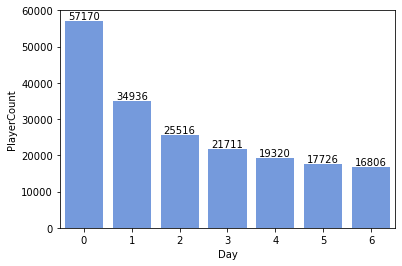
\includegraphics[width=0.7\textwidth]{figures/evaluation/Image_PlayerChurnPeriod.png}
      \caption[新進玩家之流失速度圖]{新進玩家之流失速度圖(x 軸為玩家登入日減去創立帳號日;y 軸為有登入之玩家數)}
      \label{fig:eva_PlayerChurnPeriod}
    \end{center}
\end{figure}

本文將定義新進玩家\ (\ 於~\ref{subsec:AudienceEvaluation}~小節中,篩選後之有價值玩家\ )\ 中的非流失玩家與流失玩家。觀察期有登入紀錄的玩家中,表現期間也有登入紀錄者視為非流失玩家,反之視為流失玩家。如表~\ref{tab:ChurnPlayerAndNonChurnPlayerDefinition},會有 20,488 位非流失玩家及 36,682 位流失玩家來做後續實驗。

\begin{table}[!htb]
	\centering
	\begin{tabular}{ccccc}
	\hline \hline
	有價值玩家數 & 非流失玩家 & 非流失玩家佔比 & 流失玩家數 & 流失玩家佔比 \\
    \hline \hline
    57,170 & 20,488 & 35.84 \% & 36,682 & 64.16 \% \\
    \hline \hline
	\end{tabular}
	\caption[非流失玩家及流失玩家定義表]{非流失玩家及流失玩家定義表}
	\label{tab:ChurnPlayerAndNonChurnPlayerDefinition}
\end{table}
\newpage

從原始資料集中探勘出$O$天\ (\ 資料特徵探勘期,即觀察期\ )\ 內之資料特徵,並透過特徵工程進行轉化。以多種統計方式,並拆分多個時間段,產生第一層特徵變數,再對第一層特徵變數做計算,進而得到第二層特徵變數。原本探勘出 23 個特徵,經過特徵工程後,最後共得到了 251 個特徵變數。

另外,因類別型資料特徵不適用於樹狀結構之學習模型,故在其應用於機器學習前,將此類資料特徵透過One Hot Encoding進行轉化,以利機器學習訓練,將其也歸類至第一層特徵,如圖~\ref{fig:eva_OneHotEncoder}。

\begin{figure}[!htb]
    \begin{center}
      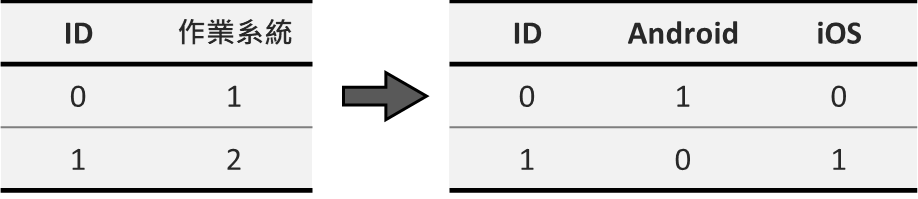
\includegraphics[width=0.75\textwidth]{figures/evaluation/Image_OneHotEncoder.png}
      \caption[One Hot Encoding 示意圖]{One Hot Encoding 示意圖 (作業系統1為Android;2為iOS)}
      \label{fig:eva_OneHotEncoder}
    \end{center}
\end{figure}

為了避免特徵之間存在高度相關性,會影響到模型預測的準確性,本文對上述 251 個特徵變數進行篩選。透過支持向量機 ( Support Vector Machine ) 找出高共線性的冗贅特徵,並將其排除,最後只剩下 49 個特徵變數。此外,去掉高共線性的特徵也可以讓模型的可解釋性更好。表~\ref{tab:NumberOfFeatures} 為資料特徵總數表。

\begin{table}[!htb]
	\centering
	\begin{tabular}{ccccc}
	\hline \hline
	原始特徵數 & 第一層特徵數 & 第二層特徵數 & 篩選前特徵數 & 篩選後特徵數 \\
    \hline \hline
    23 & 158 & 93 & 251 & 49 \\
    \hline \hline
	\end{tabular}
	\caption[資料特徵總數表]{資料特徵總數表}
	\label{tab:NumberOfFeatures}
\end{table}

為了避免部分特徵之數值過大或過小,彼此間差距較大,會影響到模型訓練精度,本文對所有特徵數值進行歸一化 ( Normalization )。式~\ref{eq:Normalization} 為本文歸一化的方式,會將所有數值映射到 [0,1] 區間。

\begin{equation}
  \label{eq:Normalization}
  x' = \frac{x-min(x)}{max(x)-min(x)}
\end{equation}
\newpage

\section{資料分析評估}
\label{sec:DataAnalysisEvaluation}

此階段將評估前章 \ref{subsubsec:ValuableFeatures}~小節之高資訊量資料特徵推測,於 \ref{subsec:EDAEvaluation}~小節\ 探索性資料分析評估說明。

\subsection{探索性資料分析評估}
\label{subsec:EDAEvaluation}

利用長條圖觀察設備所在地,如圖~\ref{fig:eva_CountryBarPlot} 及圖~\ref{fig:eva_CountryPayerRatioBarPlot},從兩圖中可以看出,Country 3的玩家數最多,但其付費玩家比例則偏低,可見雖有大量的玩家遊玩,卻無法提升其付費意願;而Country 4的玩家數雖不突出,但其付費玩家比例則最高,可見於該地之玩家相較於Country 3有更高的付費意願,可能是因為環境或消費行為不同所造成,所以相較於提升玩家數,更重要的是在於如何提高玩家付費意願。

\begin{figure}[!htb]
    \begin{center}
      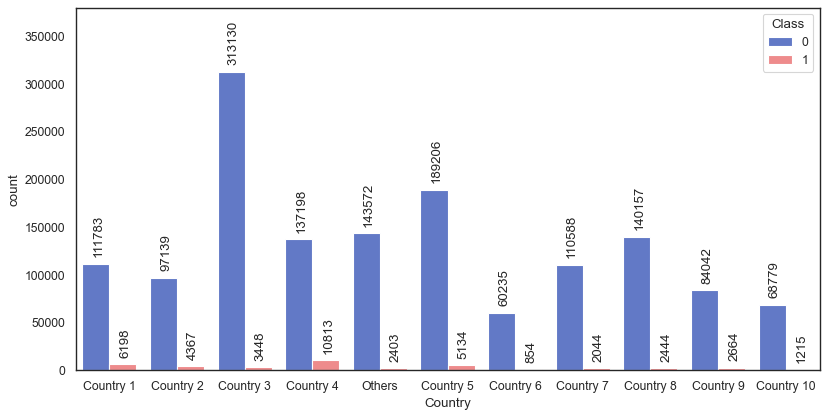
\includegraphics[width=1\textwidth]{figures/evaluation/Image_CountryBarPlot.png}
      \caption[觀察設備所在地之付費玩家與非付費玩家數量長條圖]{觀察設備所在地之付費玩家與非付費玩家數量長條圖\ (\ x 軸為設備所在地;y 軸為玩家數量\ )\ }
      \label{fig:eva_CountryBarPlot}
    \end{center}
\end{figure}
\newpage

\begin{figure}[!htb]
    \begin{center}
      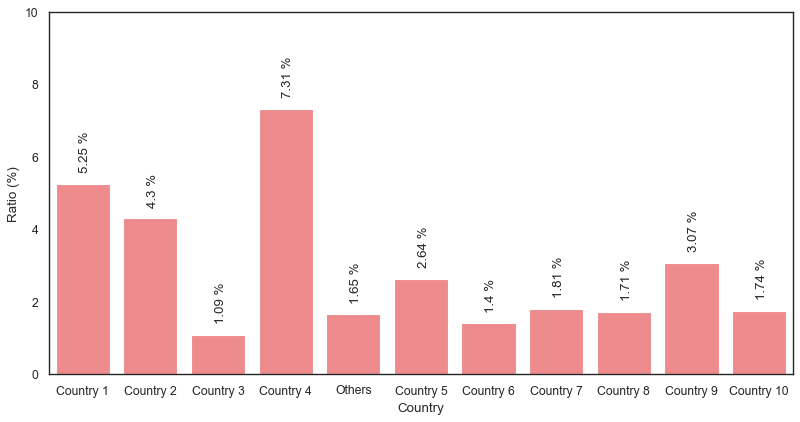
\includegraphics[width=1\textwidth]{figures/evaluation/Image_CountryPayerRatioBarPlot.png}
      \caption[觀察設備所在地之付費玩家比例長條圖]{觀察設備所在地之付費玩家比例長條圖\ (\ x 軸為設備所在地;y 軸為付費玩家比例\ )\ }
      \label{fig:eva_CountryPayerRatioBarPlot}
    \end{center}
\end{figure}

利用長條圖觀察在資料集中是否有不合適之資料特徵存在,如圖~\ref{fig:eva_UnreasonableFeatureBarPlot},該圖為GameTypeE 59遊戲之總贏遊戲次數,從圖中可以看出,僅有付費玩家有數值,而非付費玩家則全數皆為0,造成此種現象之原因為因為該款遊戲僅有付費玩家可以遊玩,故將不適合當作資料特徵,予以刪除。

\begin{figure}[!htb]
    \begin{center}
      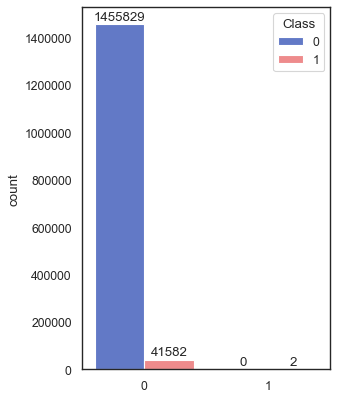
\includegraphics[width=0.4\textwidth]{figures/evaluation/Image_UnreasonableFeatureBarPlot.png}
      \caption[觀察GameTypeE 59號遊戲之總贏遊戲次數長條圖]{觀察GameTypeE 59號遊戲之總贏遊戲次數長條圖\ (\ x 軸為總贏遊戲次數;y 軸為玩家數量\ )\ }
      \label{fig:eva_UnreasonableFeatureBarPlot}
    \end{center}
\end{figure}
\newpage

利用散佈圖觀察在資料集中的高資訊量資料特徵,如圖~\ref{fig:eva_ValuableFeatureScatterPlot_GameTypeA} (a) 及圖~\ref{fig:eva_ValuableFeatureScatterPlot_GameTypeA} (b),該圖組為GameTypeA之總贏分與遊戲貨幣A之餘額變化,從兩圖中可以看出,付費玩家與非付費玩家之分佈有明顯差異,推測可以帶給學習模型很好的分類資訊。

\begin{figure}[!htb]
    \centering
    \subfigure[總贏分散佈圖\ (\ x 軸為非付費玩家與付費玩家;y 軸為總贏分\ )\ ] {
      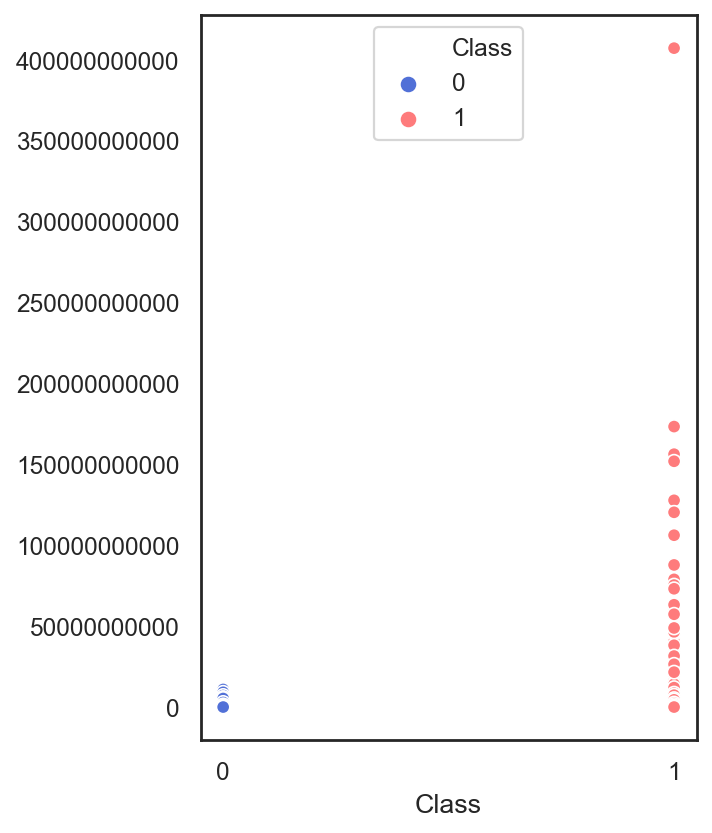
\includegraphics[width=0.45\columnwidth]{figures/evaluation/Image_GameTypeATotalWin.png}
    }
    \subfigure[遊戲貨幣A之餘額變化散佈圖\ (\ x 軸為非付費玩家與付費玩家;y 軸為遊戲貨幣A之餘額變化\ )\ ] {
        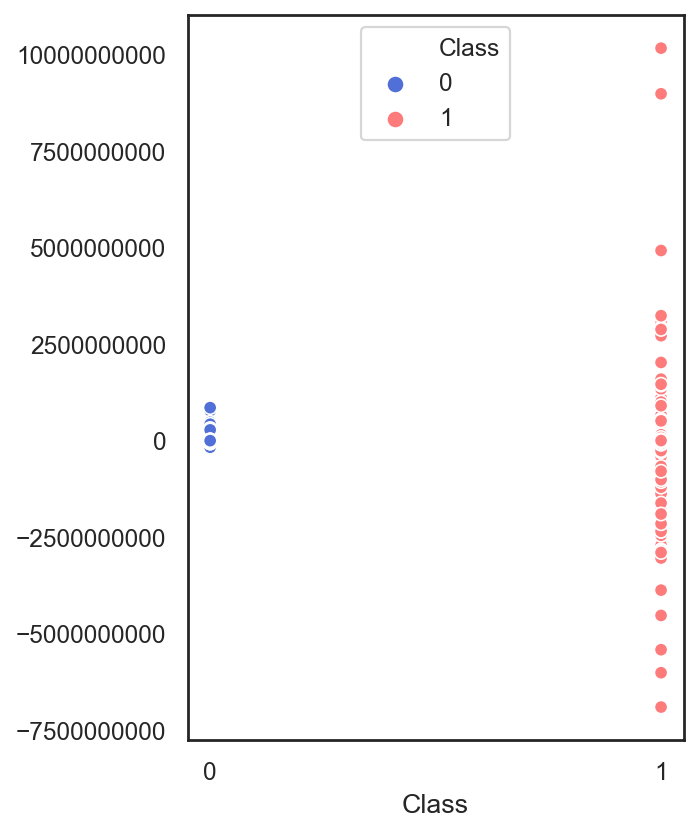
\includegraphics[width=0.45\columnwidth]{figures/evaluation/Image_GameTypeABalanceDiff.png}
    }
    \caption[觀察GameTypeA資料特徵散佈圖]{觀察GameTypeA資料特徵散佈圖}
    \label{fig:eva_ValuableFeatureScatterPlot_GameTypeA}
\end{figure}
\newpage

圖~\ref{fig:eva_ValuableFeatureScatterPlot_GameTypeAWithEntered} (a) 及圖~\ref{fig:eva_ValuableFeatureScatterPlot_GameTypeAWithEntered} (b),該圖組為GameTypeA之遊玩天數與總贏分、遊戲貨幣A之餘額變化,從兩圖中可以看出,隨著遊玩天數的增加,數值的差異性則拉大,推測可以帶給學習模型很好的分類資訊。

\begin{figure}[!htb]
    \centering
    \subfigure[遊玩天數與總贏分散佈圖\ (\ x 軸為遊玩天數;y 軸為總贏分\ )\ ] {
      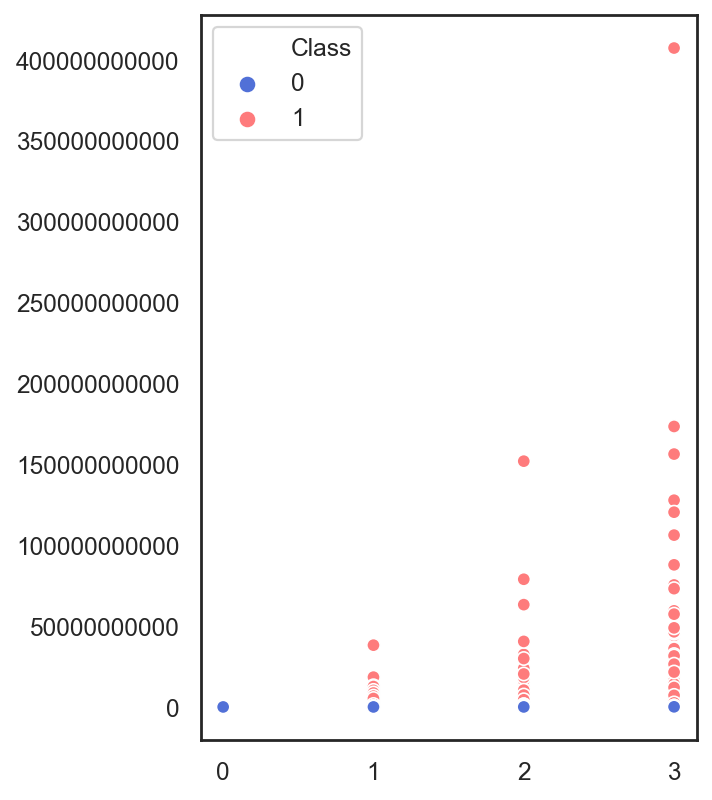
\includegraphics[width=0.45\columnwidth]{figures/evaluation/Image_GameTypeATotalWin&Entered.png}
    }
    \subfigure[遊玩天數與遊戲貨幣A之餘額變化散佈圖\ (\ x 軸為遊玩天數;y 軸為遊戲貨幣A之餘額變化\ )\ ] {
        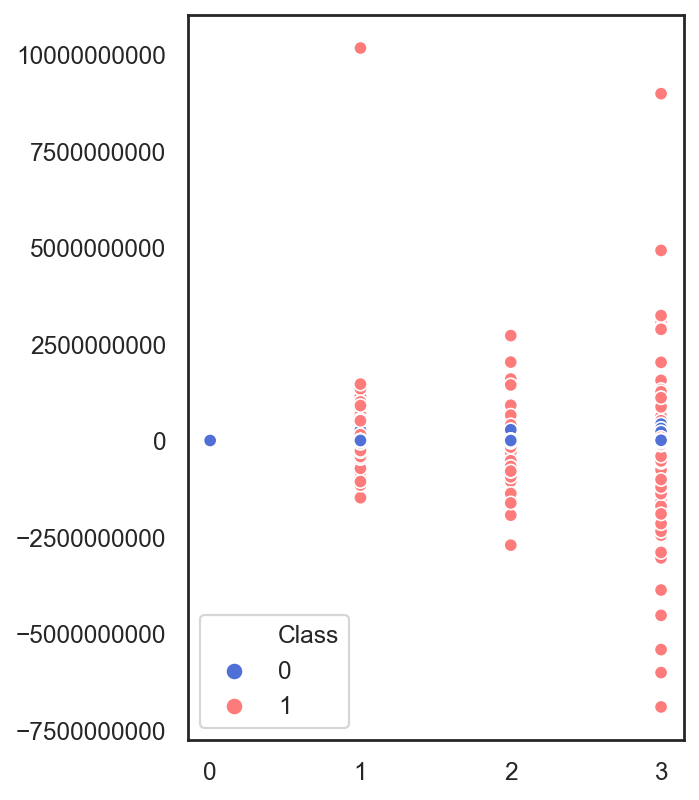
\includegraphics[width=0.45\columnwidth]{figures/evaluation/Image_GameTypeABalanceDiff&Entered.png}
    }
    \caption[觀察GameTypeA資料特徵關聯散佈圖]{觀察GameTypeA資料特徵關聯散佈圖}
    \label{fig:eva_ValuableFeatureScatterPlot_GameTypeAWithEntered}
\end{figure}
\newpage

圖~\ref{fig:eva_ValuableFeatureScatterPlot_GameTypeD65} (a) 及圖~\ref{fig:eva_ValuableFeatureScatterPlot_GameTypeD65} (b),該圖組為GameTypeD 65號遊戲之總贏分與總贏遊戲次數,從兩圖中可以看出,付費玩家與非付費玩家之分佈明顯無差異,推測無法帶給學習模型很好的分類資訊。

\begin{figure}[!htb]
    \centering
    \subfigure[總贏分散佈圖\ (\ x 軸為非付費玩家與付費玩家;y 軸為總贏分\ )\ ] {
      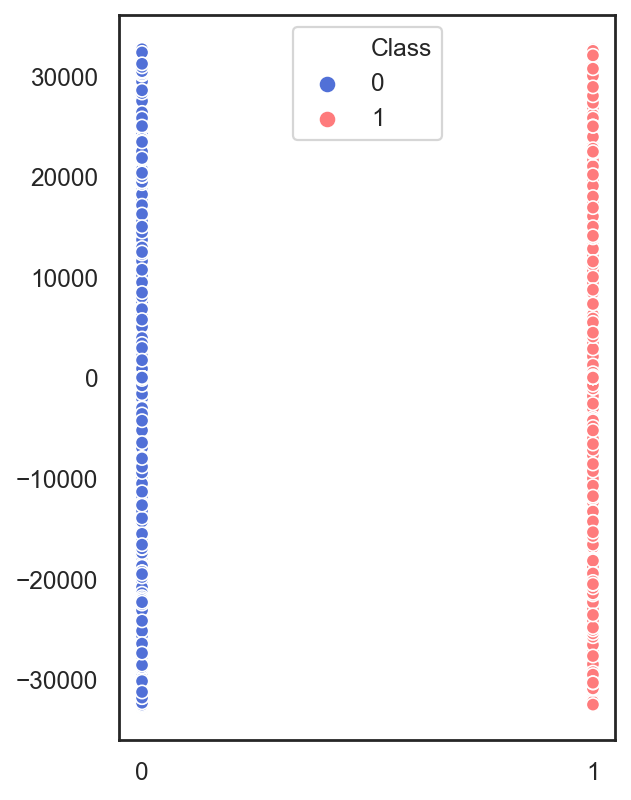
\includegraphics[width=0.45\columnwidth]{figures/evaluation/Image_GameTypeD65TotalWin.png}
    }
    \subfigure[總贏遊戲次數散佈圖\ (\ x 軸為非付費玩家與付費玩家;y 軸為總贏遊戲次數\ )\ ] {
        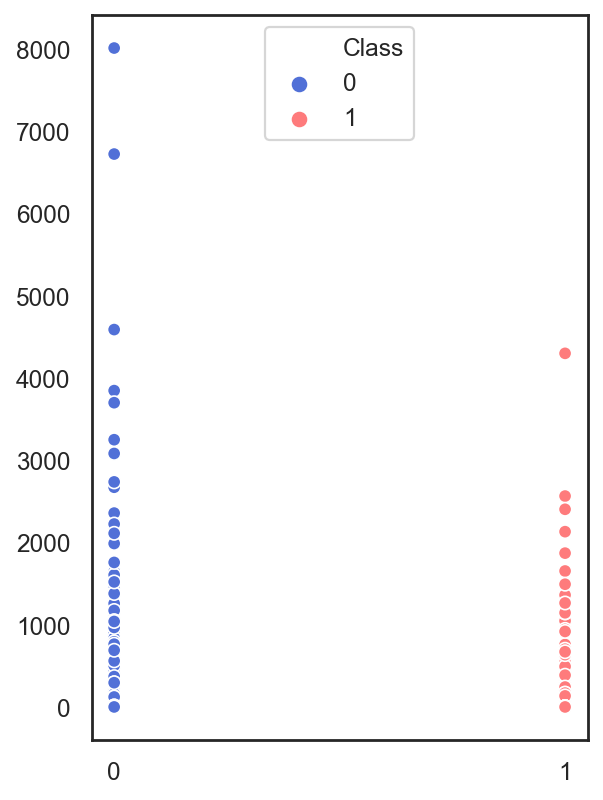
\includegraphics[width=0.45\columnwidth]{figures/evaluation/Image_GameTypeD65TotalWinTimes.png}
    }
    \caption[觀察GameTypeD 65號遊戲資料特徵關聯散佈圖]{觀察GameTypeD 65號遊戲資料特徵關聯散佈圖}
    \label{fig:eva_ValuableFeatureScatterPlot_GameTypeD65}
\end{figure}
\newpage

圖~\ref{fig:eva_ValuableFeatureBarPlot_GameTypeE62TotalWinTimes},該圖為GameTypeE 62號遊戲之總贏遊戲次數,從圖中可以看出,在贏遊戲次數偏低時,非付費玩家佔了大多數,而付費玩家則相對偏少,推測可以帶給學習模型很好的分類資訊。

\begin{figure}[!htb]
    \begin{center}
      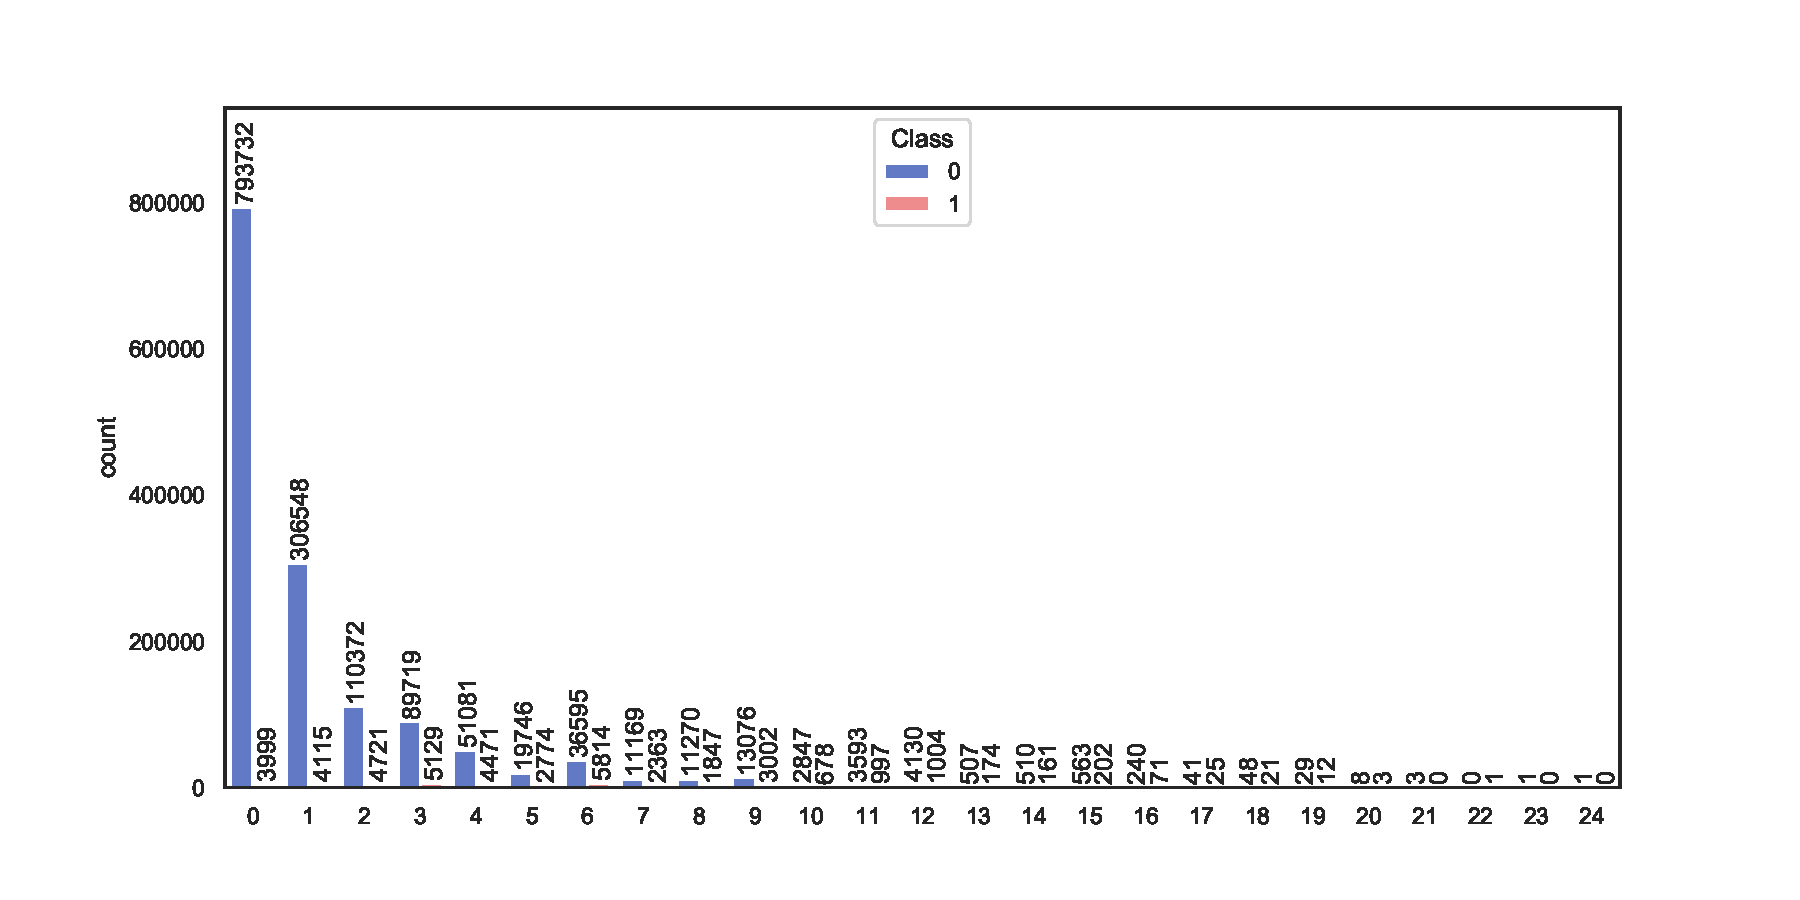
\includegraphics[width=1\textwidth]{figures/evaluation/Image_GameTypeE62TotalWinTimes.pdf}
      \caption[觀察GameTypeE 62號遊戲之總贏遊戲次數長條圖]{觀察GameTypeE 62號遊戲之總贏遊戲次數長條圖\ (\ x 軸為總贏遊戲次數;y 軸為玩家數量\ )\ }
      \label{fig:eva_ValuableFeatureBarPlot_GameTypeE62TotalWinTimes}
    \end{center}
\end{figure}

圖~\ref{fig:eva_ValuableFeatureScatterPlot_GameTyeE62TotalCoinAAwarded},該圖為GameTypeE 62號遊戲之獲得遊戲貨幣A之總額,從圖中可以看出,付費玩家資料分佈較廣,而非付費玩家則侷限在10,000左右,推測可以帶給學習模型很好的分類資訊。

\begin{figure}[!htb]
    \begin{center}
      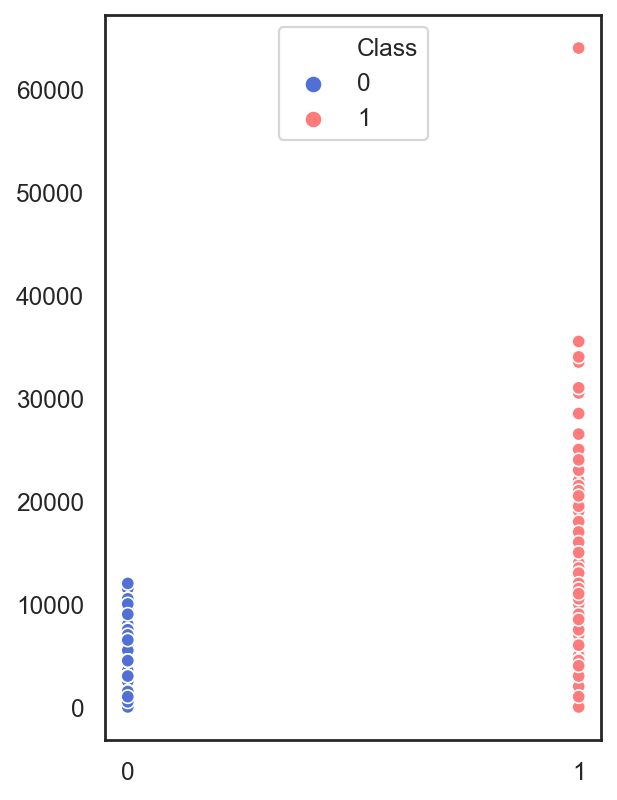
\includegraphics[width=0.4\textwidth]{figures/evaluation/Image_GameTypeE62TotalCoinAAwarded.png}
      \caption[觀察GameTypeE 62號遊戲之獲得遊戲貨幣A之總額散佈圖]{觀察GameTypeE 62號遊戲之獲得遊戲貨幣A之總額散佈圖\ (\ x 軸為非付費玩家與付費玩家;y 軸為獲得遊戲貨幣A之總額\ )\ }
      \label{fig:eva_ValuableFeatureScatterPlot_GameTyeE62TotalCoinAAwarded}
    \end{center}
\end{figure}
\newpage

\section{機器學習評估}
\label{sec:MachineLearningEvaluation}

此階段將評估前章~\ref{sec:MachineLearning} 小節之機器學習。~\ref{subsec:SplitDatasetEvaluation} 小節為分割訓練與測試資料集評估,將說明~\ref{subsec:SplitDataset} 小節之分割訓練與測試資料集;~\ref{subsec:ImbalancedDataHandleEvaluation} 小節為不平衡資料權重調整評估,將說明~\ref{subsec:ImbalancedDataHandle} 小節之不平衡資料權重調整;~\ref{subsec:BestModelEvaluation} 小節為最佳模型評估,將說明~\ref{subsec:TuningBestParams} 小節之搜尋最佳參數解、~\ref{subsec:CrossValidation} 小節之交叉驗證及~\ref{subsec:EvaluateBestModel} 小節之評估驗證最佳模型。

\subsection{分割訓練與測試資料集評估}
\label{subsec:SplitDatasetEvaluation}

將資料集依照 8:2 之比例分割。如圖~\ref{fig:Image_SplitDataset},採分類隨機抽樣,即流失玩家與非流失玩家各別以 8:2 之比例隨機抽樣。表~\ref{tab:NumberOfSplitedPayerAndNonPayer} 為分割完資料集後之流失玩家數與非流失玩家數,訓練資料集與測試資料集之流失玩家與非流失玩家比例皆與原資料集相等,約為 1.79 倍。

\begin{table}[!htb]
	\centering
	\begin{tabular}{|c|r|r|}
	\hline \hline
	\diagbox{資料集}{玩家數} & 流失玩家 & 非流失玩家 \\
    \hline \hline
    訓練集 & 29,346 & 16,390 \\
    \hline
    測試集 & 7,336 & 4,098 \\
    \hline \hline
	\end{tabular}
	\caption[訓練與測試資料集玩家數表]{訓練與測試資料集玩家數表}
	\label{tab:NumberOfSplitedPayerAndNonPayer}
\end{table}
\newpage

\subsection{資料不平衡處理評估}
\label{subsec:ImbalancedDataHandleEvaluation}

依照式~\ref{eq:SampleWeightFormula} 計算非流失玩家樣本之放大權重,如式~\ref{eq:SampleWeightCalculation},最後將非付費玩家之樣本權重放大1.79倍。以下將進行學習模型之評估,其中將藉由混淆矩陣 ( Confusion Matrix )、精確率 ( Precision )、召回率 ( Recall )、真陽率 ( True Positive Rate, TPR ) 及假陽率 ( False Positive Rate, FPR ) 來說明評估,計算方式分別如表~\ref{tab:ConfusionMatrix}、式~\ref{eq:PrecisionFormula}、式~\ref{eq:RecallFormula}、式~\ref{eq:TPRFormula} 及式~\ref{eq:FPRFormula}。

\begin{equation}
    \label{eq:SampleWeightCalculation}
    class\ 0 : class\ 1 = \frac{29,346}{16,390} : 1 = 1.79 : 1
\end{equation}

\begin{table}[!htb]
	\centering
	\begin{tabular}{|c|c|c|}
	\hline
	& True $class\ 1$ & True $class\ 0$ \\
    \hline
    Predicted $class\ 1$ & $True\ Positive\ (\ TP\ )$ & $False\ Positive\ (\ FP\ )$ \\
    \hline
    Predicted $class\ 0$ & $False\ Negative\ (\ FN\ )$ & $True\ Negative\ (\ TN\ )$ \\
    \hline
	\end{tabular}
	\caption[混淆矩陣]{混淆矩陣}
	\label{tab:ConfusionMatrix}
\end{table}

\begin{equation}
    \label{eq:PrecisionFormula}
    Precision = \frac{TP}{TP + FP}
\end{equation}

\begin{equation}
    \label{eq:RecallFormula}
    Recall = \frac{TP}{TP + FN}
\end{equation}

\begin{equation}
    \label{eq:TPRFormula}
    True\ Positive\ Rate\ (\ TPR\ ) = \frac{TP}{TP + FN} = Recall
\end{equation}

\begin{equation}
    \label{eq:FPRFormula}
    False\ Positive\ Rate\ (\ FPR\ ) = \frac{FP}{TN + FP}
\end{equation}
\newpage

我們將藉由接收者操作特徵曲線以及精確召回曲線來觀察學習模型間的精確率、召回率、真陽率及假陽率,如圖~\ref{fig:eva_ROCCurve} 及圖~\ref{fig:eva_PRCurve}。前者於 x 軸及 y 軸皆以值越大越理想,故曲線越趨近於右上角則越佳;後者於 x 軸為值越小越理想、y 軸為值越大越理想,故曲線越趨近於左上角則越佳。將再分別利用 AUC ( Area Under Curve ) 及 AP ( Average Precision ) 來衡量兩曲線,皆為計算該曲線面積。

\begin{figure}[!htb]
    \begin{center}
      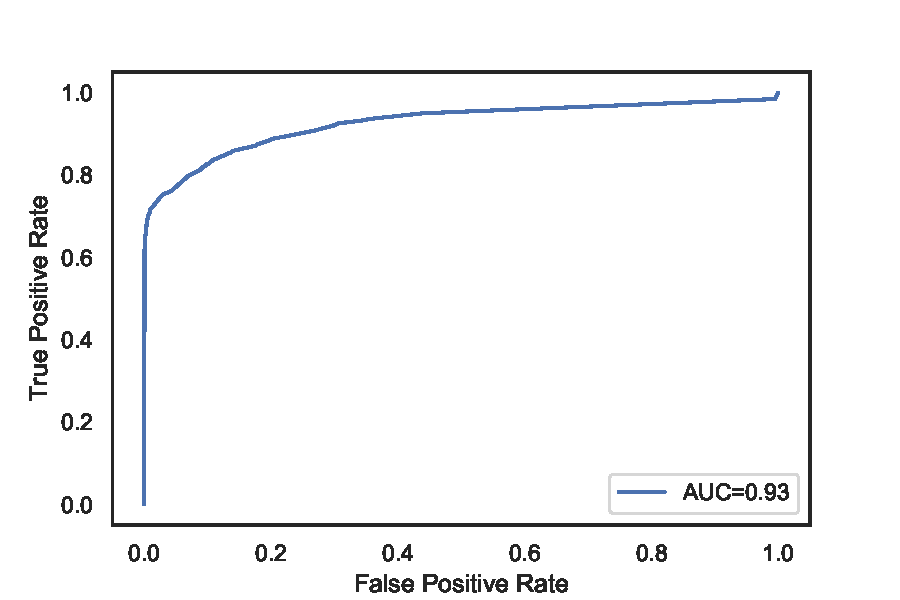
\includegraphics[width=0.7\textwidth]{figures/evaluation/Image_ROCCurve.pdf}
      \caption[接收者操作特徵曲線示意圖]{接收者操作特徵曲線示意圖\ (\ x 軸為假陽率;y 軸為真陽率;AUC為其曲線面積\ )}
      \label{fig:eva_ROCCurve}
    \end{center}
\end{figure}

\begin{figure}[!htb]
    \begin{center}
      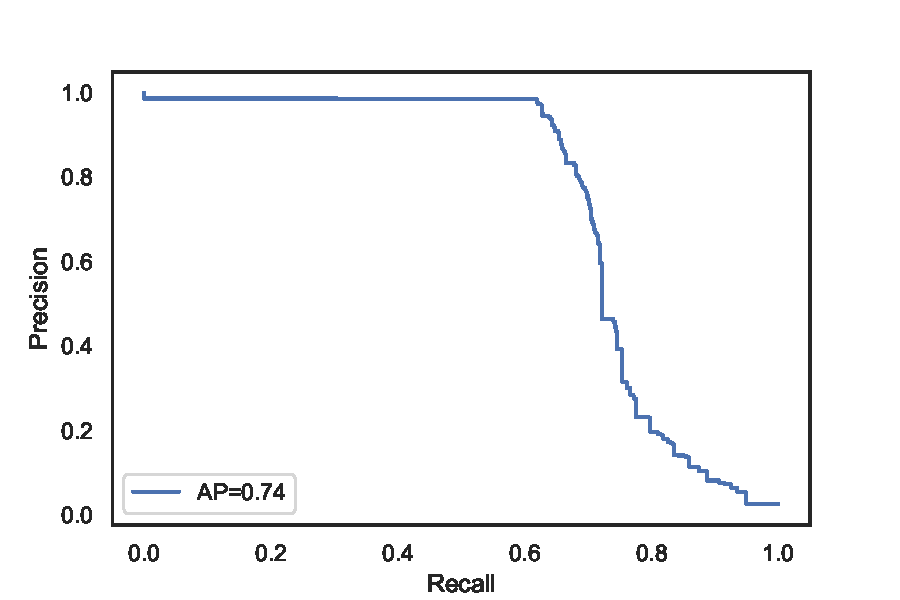
\includegraphics[width=0.7\textwidth]{figures/evaluation/Image_PRCurve.pdf}
      \caption[精確召回曲線示意圖]{精確召回曲線示意圖\ (\ x 軸為召回率;y 軸為精確率;AP 為其曲線面積\ )}
      \label{fig:eva_PRCurve}
    \end{center}
\end{figure}
\newpage

本論文將以評估精確召回曲線為重,因在不平衡資料集上進行評估時,接收者操作特徵曲線將無法準確的呈現出學習模型的好壞,常有在接收者操作特徵曲線上表現良好,但其精確召回曲線卻不如預期,導致此情況原因為多數群之評估遠大於少數群之評估,故可在接收者操作特徵曲線上擁有好的數值,卻在精確召回曲線中表現不佳\cite{davis2006relationship},如圖~\ref{fig:eva_GoodROCBadPR}。

\begin{figure}[!htb]
    \begin{center}
      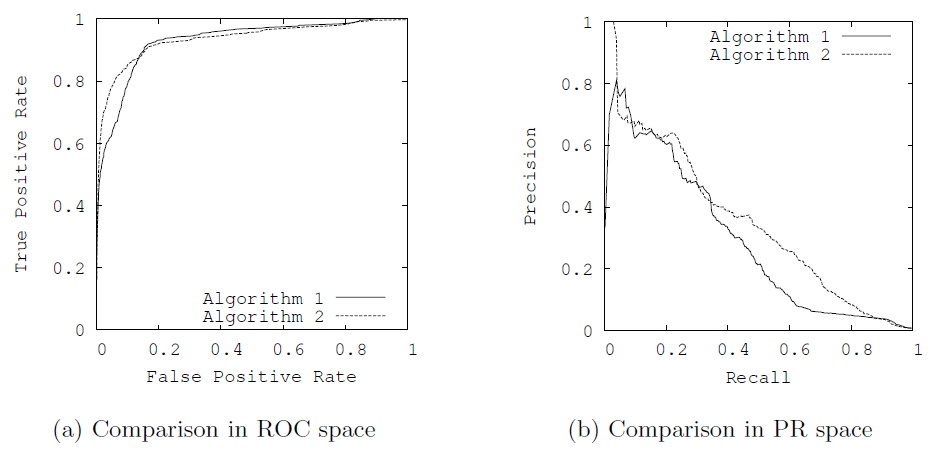
\includegraphics[width=1\textwidth]{figures/evaluation/Image_GoodROCBadPR.png}
      \caption[不平衡資料中接收者操作特徵曲線失準示意圖]{不平衡資料中接收者操作特徵曲線失準示意圖\ (\ 此圖取自~\cite{davis2006relationship}\ )}
      \label{fig:eva_GoodROCBadPR}
    \end{center}
\end{figure}
\newpage

圖~\ref{fig:eva_ROCCurveEvaluationImbalancedData} 為三種學習模型之接收者操作特徵曲線,並比較不平衡資料處理前後之差異,(a)為決策樹、(b)為隨機森林、(c)為極限梯度提升,藍色線為未加入權重值、紅色底為加入權重值,從圖組中可以看出,在流失玩家之樣本權重上進行放大,有助於學習模型之分類,使預設更加準確。AUC最高值於極限梯度提升加入權重值,為0.95。

\begin{figure}[!htb]
    \centering
    \subfigure[Decision Tree ROC Curve圖] {
      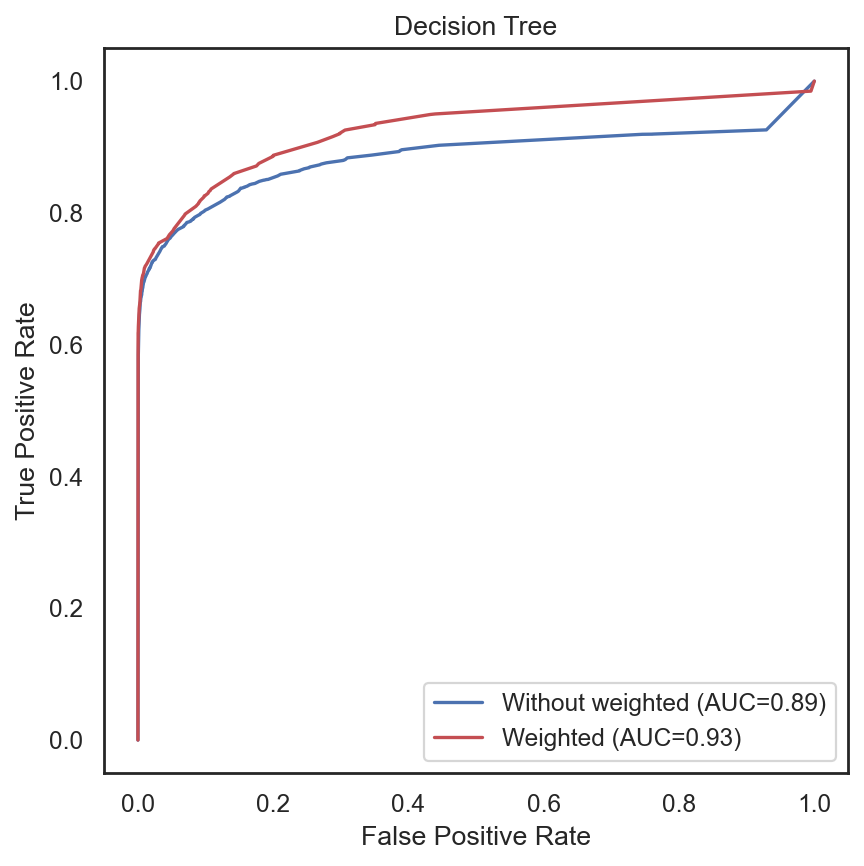
\includegraphics[width=0.47\columnwidth]{figures/evaluation/Image_DTROCCurve.png}
    }
    \subfigure[Random Forest ROC Curve圖] {
        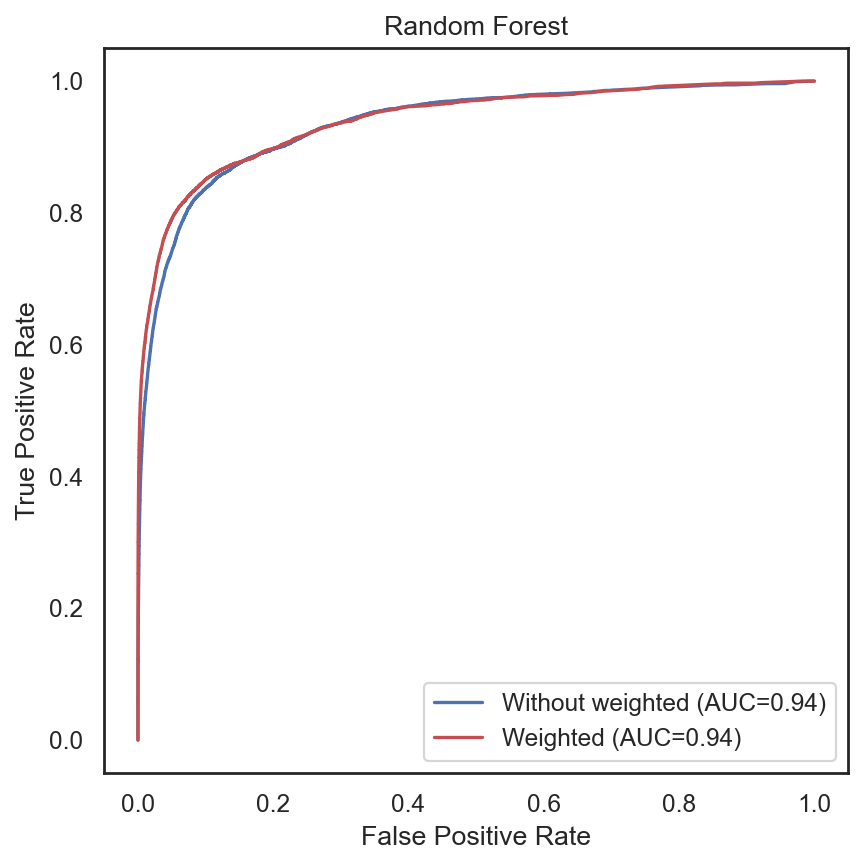
\includegraphics[width=0.47\columnwidth]{figures/evaluation/Image_RFROCCurve.png}
    }
    \subfigure[XGBoost ROC Curve圖] {
        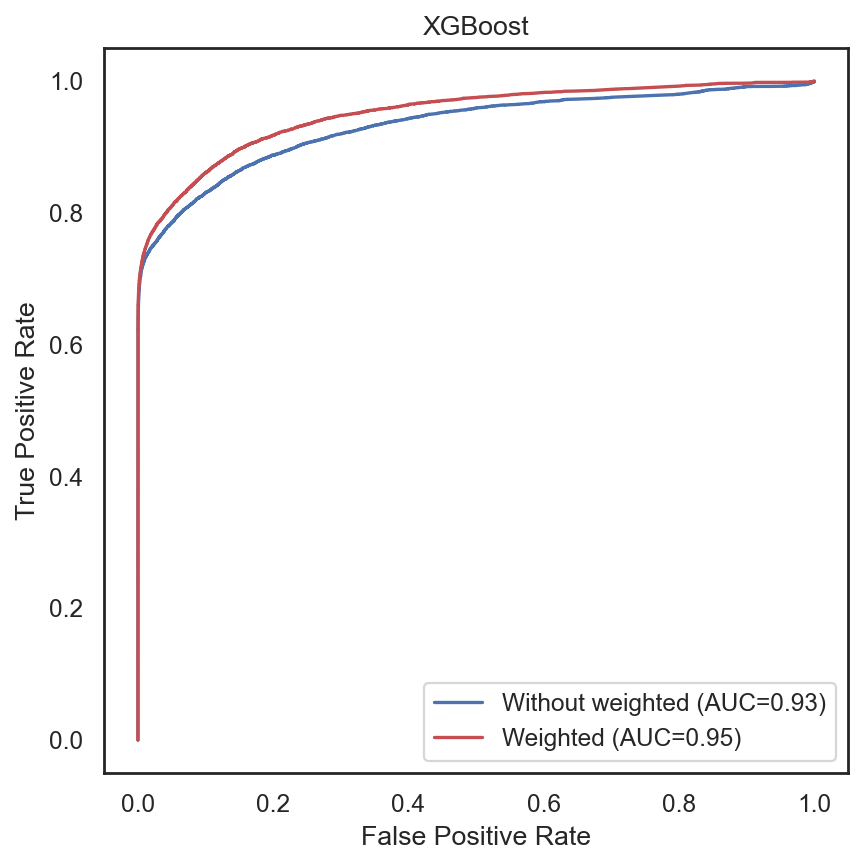
\includegraphics[width=0.47\columnwidth]{figures/evaluation/Image_XGBROCCurve.png}
    }
    \caption[不平衡資料處理前後比較之接收者操作特徵曲線圖]{不平衡資料處理前後比較之接收者操作特徵曲線圖\ (\ x 軸為假陽率;y 軸為真陽率\ )}
    \label{fig:eva_ROCCurveEvaluationImbalancedData}
\end{figure}
\newpage

圖~\ref{fig:eva_PRCurveEvaluationImbalancedData} 為三種學習模型之精確召回曲線,並比較不平衡資料處理前後之差異,(a)為決策樹、(b)為隨機森林、(c)為極限梯度提升,藍色線為未加入權重值、紅色底為加入權重值,從圖組中可以看出,在流失玩家之樣本權重上進行放大,有助於學習模型之分類,使預設更加準確。AP最高值於極限梯度提升加入權重值,為0.79。

\begin{figure}[!htb]
    \centering
    \subfigure[Decision Tree PR Curve圖] {
      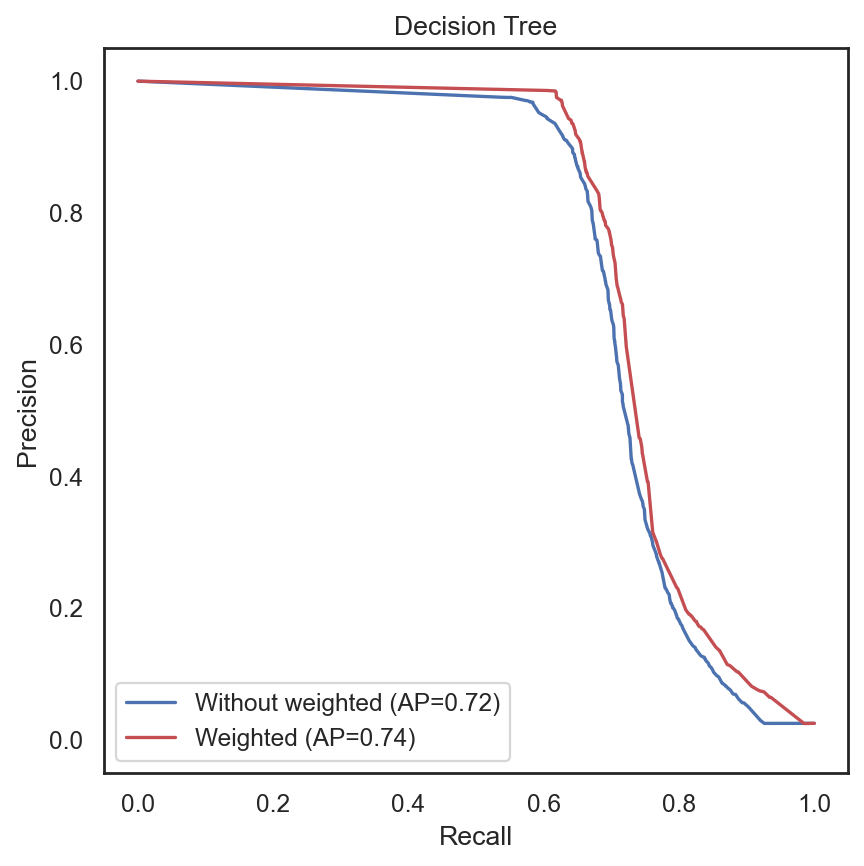
\includegraphics[width=0.47\columnwidth]{figures/evaluation/Image_DTPRCurve.png}
    }
    \subfigure[Random Forest PR Curve圖] {
        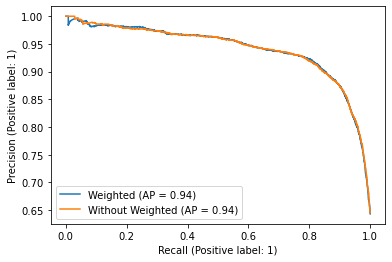
\includegraphics[width=0.47\columnwidth]{figures/evaluation/Image_RFPRCurve.png}
    }
    \subfigure[XGBoost PR Curve圖] {
        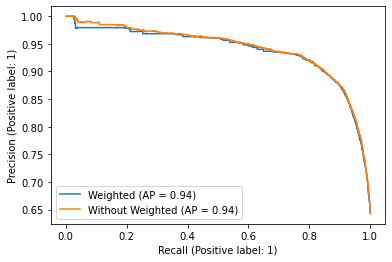
\includegraphics[width=0.47\columnwidth]{figures/evaluation/Image_XGBPRCurve.png}
    }
    \caption[不平衡資料處理前後比較之精確召回曲線圖]{不平衡資料處理前後比較之精確召回曲線圖\ (\ x 軸為召回率;y 軸為精確率\ )}
    \label{fig:eva_PRCurveEvaluationImbalancedData}
\end{figure}

上述兩種評估方式皆為在加入權重值後,改進了學習模型的訓練,使其不受於資料不平衡之影響,且適用於三種學習模型。
\newpage

\subsection{最佳模型評估}
\label{subsec:BestModelEvaluation}

利用交叉驗證來調教出最佳模型。如圖~\ref{fig:Image_RepeatedStratifiedKFold},我們將採用Reapted 2次及5-Fold,最後使用測試資料集進行評估驗證,將說明 7,336 位流失玩家 ( $class\ 1$ ) 及 4,098 位非流失玩家 ( $class\ 0$ )。驗證結果如表~\ref{tab:BestModelEvaluation},從表中可以看出,極限梯度提升的 Weighted F$_{\beta}$ - Score 為三者最高,預測能力最佳。

\begin{table}[!htb]
    \centering
        \begin{tabular}{|c|r|r|r|r|}
            \hline \hline
            \multirow{2}*{\diagbox{學習模型}{評估}} & $precision^+$ & $recall^+$ & ${F_{beta}}^+$ & \multirow{2}*{$Weighted\ F_{beta}$} \\
            \cline{2-4}
            & $precision^-$ & $recall^-$ & ${F_{beta}}^-$ & \\
            \hline \hline
            \multirow{2}*{決策樹} & 0.700 & 0.726 & 0.726 & \multirow{2}*{0.985} \\
            \cline{2-4}
            & 0.993 & 0.992 & 0.992 & \\
            \hline
            \multirow{2}*{隨機森林} & 0.840 & 0.678 & 0.678 & \multirow{2}*{0.989} \\
            \cline{2-4}
            & 0.992 & 0.997 & 0.997 & \\
            \hline
            \multirow{2}*{極限梯度提升} & 0.965 & 0.722 & 0.723 & \multirow{2}*{0.992} \\
            \cline{2-4}
            & 0.993 & 0.999 & 0.999 & \\
            \hline
            \multicolumn{5}{|l|}{$+$:以正例(流失玩家 $class\ 1$ )為評估對象進行計算} \\
            \multicolumn{5}{|l|}{$-$:以反例(非流失玩家 $class\ 0$ )為評估對象進行計算} \\
            \hline \hline
        \end{tabular}
    \caption[最佳模型評估表]{最佳模型評估表}
    \label{tab:BestModelEvaluation}
\end{table}

圖~\ref{fig:eva_ModelsROCCurve} 及圖~\ref{fig:eva_ModelsPRCurve} 為三種學習模型之接收者操作特徵曲線及精確召回曲線比較圖,並且都為加入權重值之結果,從圖組中可以看出,皆為極限梯度提升擁有最好的結果,綜合上述得到的實驗結果,我們認為極限梯度提升非常適用於遊戲領域巨量資料預測分類上,因其提升方法建樹,強化修正於分類錯誤樣本,有效的提升學習模型預測之準確度,並採用梯度下降法 ( Gradient Descent ) 來加速學習模型之收斂,減少建樹時間成本。

%另外,此處實驗之Random Forest遭遇了前述所提到ROC Curve表現佳,卻在PR Curve表現差的問題,甚至評估結果差於基礎學習模型Decision Tree,有可能是因學習模型有過擬合 ( Overfitting ) 的情形發生,所導致PR Curve表現不佳。
\newpage

\begin{figure}[!htb]
    \begin{center}
      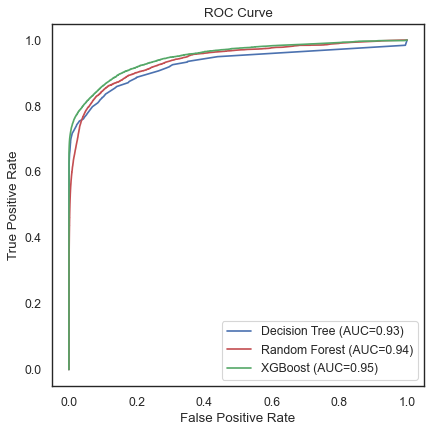
\includegraphics[width=0.6\textwidth]{figures/evaluation/Image_ModelsROCCurve.png}
      \caption[三種學習模型之ROC Curve比較圖]{三種學習模型之ROC Curve比較圖}
      \label{fig:eva_ModelsROCCurve}
    \end{center}
\end{figure}

\begin{figure}[!htb]
    \begin{center}
      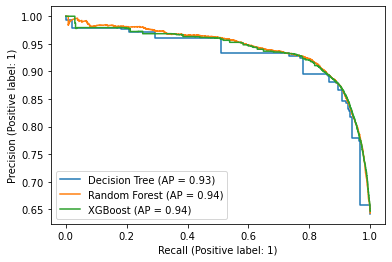
\includegraphics[width=0.6\textwidth]{figures/evaluation/Image_ModelsPRCurve.png}
      \caption[三種學習模型之PR Curve比較圖]{三種學習模型之PR Curve比較圖}
      \label{fig:eva_ModelsPRCurve}
    \end{center}
\end{figure}
\newpage

表~\ref{tab:BestModelParams} 為三種學習模型之最佳參數解,參數搜尋範圍如表~\ref{tab:ParamsSearchRange},決策樹因其為單樹結構,相較之下需要生成更深的樹;而隨機森林及極限梯度提升則因其為多樹結構,希望能以廣度發展,而非深度,相較之下需要生成更多的樹。

\begin{table}[!htb]
    \centering
        \begin{tabular}{clll}
            \hline \hline
            學習模型 & Decision Tree & Random Forest & XGBoost \\
            \hline \hline
            \multirow{4}*{參數調教} & max\char`_depth=13 & n\char`_estimators=55 & n\char`_estimators=55 \\
            & min\char`_samples\char`_split=2 & max\char`_depth=13 & max\char`_depth=10 \\
            & min\char`_samples\char`_leaf=5 & min\char`_samples\char`_split=2 & \\
            && min\char`_samples\char`_leaf=5 & \\
            \hline \hline
        \end{tabular}
    \caption[最佳模型參數解表]{最佳模型參數解表}
    \label{tab:BestModelParams}
\end{table}

\begin{table}[!htb]
    \centering
        \begin{tabular}{cl}
            \hline \hline
            參數名 & 搜尋範圍 \\
            \hline \hline
            n\char`_estimators & 20, 25, 30, 35, 40, 45, 50, 55, 60 \\
            \hline
            max\char`_depth & 1, 2, 3, 4, 5, 6, 7, 8, 9, 10, 11, 12, 13, 14, 15 \\
            \hline
            min\char`_samples\char`_split & 2, 4, 6, 8, 10 \\
            \hline
            min\char`_samples\char`_leaf & 1, 5, 10, 15, 20 \\
            \hline \hline
        \end{tabular}
    \caption[參數搜尋範圍表]{參數搜尋範圍表}
    \label{tab:ParamsSearchRange}
\end{table}
\newpage

\section{預測結果分析評估}
\label{sec:PredictionResultAnalysisEvaluation}

此階段將評估前章~\ref{sec:PredictionResultAnalysis} 小節之預測結果分析。~\ref{subsec:FeatureImportanceEvaluation} 小節為資料特徵重要性評估,將說明~\ref{subsec:FeatureImportanceAnalysis} 小節之資料特徵重要性分析。

\subsection{資料特徵重要性評估}
\label{subsec:FeatureImportanceEvaluation}

將利用式~\ref{eq:GiniImportanceFormula}、式~\ref{eq:SingleTreeFeatureImportanceFormula} 及式~\ref{eq:ModelFeatureImportanceFormula} 計算之各資料特徵於各模型之資料特徵重要性。如圖~\ref{fig:eva_DTFeatureImportances}、圖~\ref{fig:eva_RFFeatureImportances} 及圖~\ref{fig:eva_XGBFeatureImportances},分別為決策樹、隨機森林及極限梯度提升之資料特徵重要性比較圖。

\begin{figure}[!htb]
    \begin{center}
      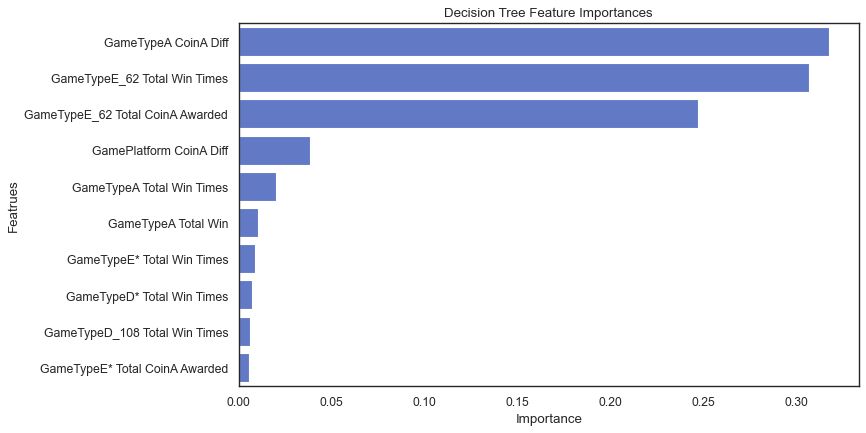
\includegraphics[width=1\textwidth]{figures/evaluation/Image_DTFeatureImportances.png}
      \caption[決策樹資料特徵重要性比較圖]{決策樹資料特徵重要性比較圖}
      \label{fig:eva_DTFeatureImportances}
    \end{center}
\end{figure}
\newpage

\begin{figure}[!htb]
    \begin{center}
      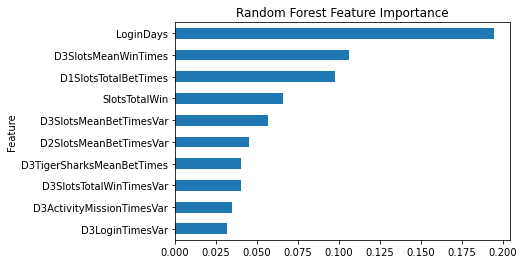
\includegraphics[width=1\textwidth]{figures/evaluation/Image_RFFeatureImportances.png}
      \caption[隨機森林資料特徵重要性比較圖]{隨機森林資料特徵重要性比較圖}
      \label{fig:eva_RFFeatureImportances}
    \end{center}
\end{figure}

\begin{figure}[!htb]
    \begin{center}
      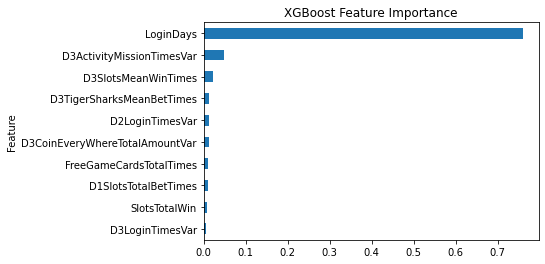
\includegraphics[width=1\textwidth]{figures/evaluation/Image_XGBFeatureImportances.png}
      \caption[極限梯度提升資料特徵重要性比較圖]{極限梯度提升資料特徵重要性比較圖}
      \label{fig:eva_XGBFeatureImportances}
    \end{center}
\end{figure}
\newpage

從三圖中可以看出,GameTypeE 62號遊戲的獲得遊戲貨幣A之總額以及總贏遊戲次數皆在三種學習模型的前四名,可以說明此款遊戲在於玩家獲得獎勵及贏得遊戲時,對於其付費意願有明顯提升;GameTypeA的遊戲貨幣A之餘額變化以及總贏分皆在前十名,可以說明此款遊戲在於玩家遊玩遊戲時的體驗起伏(無論輸或贏)及贏取分數時,對於其付費意願有明顯提升。

上述所提到的資料特徵皆在 \ref{subsubsec:ValuableFeatures}~小節中有進行推測該類資料特徵將有助於學習模型訓練,顯示先對資料進行分析,對於學習模型之解釋以及後續之利用是有相當程度上的幫助,可以透過探索性資料分析,在資料集應用於機器學習前,即先對資料進行探索,找出資料之問題或是高資訊量的資料特徵,進而增進學習模型的成效或是加強資料特徵的轉化。

另外,三種學習模型之前十名資料特徵皆為數值型的資料特徵,而無類別型資料特徵,因其資料特徵重要性之評估以計算$Gini\ Importance$為主,數值型將會比類別型來得更為顯著,未來將可在計算重要性分析中,對於不同類型的資料特徵加入權重值,使得類別型的資料特徵能夠突出,讓整體分析更加準確。

\section{產業應用分析評估}
\label{sec:ApplicationAnalysisEvaluation}

此階段將評估前章~\ref{sec:ApplicationAnalysis} 小節之產業應用分析。~\ref{subsec:SurrogateModelEvaluation} 小節為代理人模型評估,將說明~\ref{subsec:SurrogateModel} 小節之代理人模型。

\subsection{代理人模型評估}
\label{subsec:SurrogateModelEvaluation}

\newpage